\documentclass[twoside]{book}

% Packages required by doxygen
\usepackage{fixltx2e}
\usepackage{calc}
\usepackage{doxygen}
\usepackage[export]{adjustbox} % also loads graphicx
\usepackage{graphicx}
\usepackage[utf8]{inputenc}
\usepackage{makeidx}
\usepackage{multicol}
\usepackage{multirow}
\PassOptionsToPackage{warn}{textcomp}
\usepackage{textcomp}
\usepackage[nointegrals]{wasysym}
\usepackage[table]{xcolor}

% Font selection
\usepackage[T1]{fontenc}
\usepackage[scaled=.90]{helvet}
\usepackage{courier}
\usepackage{amssymb}
\usepackage{sectsty}
\renewcommand{\familydefault}{\sfdefault}
\allsectionsfont{%
  \fontseries{bc}\selectfont%
  \color{darkgray}%
}
\renewcommand{\DoxyLabelFont}{%
  \fontseries{bc}\selectfont%
  \color{darkgray}%
}
\newcommand{\+}{\discretionary{\mbox{\scriptsize$\hookleftarrow$}}{}{}}

% Page & text layout
\usepackage{geometry}
\geometry{%
  a4paper,%
  top=2.5cm,%
  bottom=2.5cm,%
  left=2.5cm,%
  right=2.5cm%
}
\tolerance=750
\hfuzz=15pt
\hbadness=750
\setlength{\emergencystretch}{15pt}
\setlength{\parindent}{0cm}
\setlength{\parskip}{3ex plus 2ex minus 2ex}
\makeatletter
\renewcommand{\paragraph}{%
  \@startsection{paragraph}{4}{0ex}{-1.0ex}{1.0ex}{%
    \normalfont\normalsize\bfseries\SS@parafont%
  }%
}
\renewcommand{\subparagraph}{%
  \@startsection{subparagraph}{5}{0ex}{-1.0ex}{1.0ex}{%
    \normalfont\normalsize\bfseries\SS@subparafont%
  }%
}
\makeatother

% Headers & footers
\usepackage{fancyhdr}
\pagestyle{fancyplain}
\fancyhead[LE]{\fancyplain{}{\bfseries\thepage}}
\fancyhead[CE]{\fancyplain{}{}}
\fancyhead[RE]{\fancyplain{}{\bfseries\leftmark}}
\fancyhead[LO]{\fancyplain{}{\bfseries\rightmark}}
\fancyhead[CO]{\fancyplain{}{}}
\fancyhead[RO]{\fancyplain{}{\bfseries\thepage}}
\fancyfoot[LE]{\fancyplain{}{}}
\fancyfoot[CE]{\fancyplain{}{}}
\fancyfoot[RE]{\fancyplain{}{\bfseries\scriptsize Generated by Doxygen }}
\fancyfoot[LO]{\fancyplain{}{\bfseries\scriptsize Generated by Doxygen }}
\fancyfoot[CO]{\fancyplain{}{}}
\fancyfoot[RO]{\fancyplain{}{}}
\renewcommand{\footrulewidth}{0.4pt}
\renewcommand{\chaptermark}[1]{%
  \markboth{#1}{}%
}
\renewcommand{\sectionmark}[1]{%
  \markright{\thesection\ #1}%
}

% Indices & bibliography
\usepackage{natbib}
\usepackage[titles]{tocloft}
\setcounter{tocdepth}{3}
\setcounter{secnumdepth}{5}
\makeindex

% Hyperlinks (required, but should be loaded last)
\usepackage{ifpdf}
\ifpdf
  \usepackage[pdftex,pagebackref=true]{hyperref}
\else
  \usepackage[ps2pdf,pagebackref=true]{hyperref}
\fi
\hypersetup{%
  colorlinks=true,%
  linkcolor=blue,%
  citecolor=blue,%
  unicode%
}

% Custom commands
\newcommand{\clearemptydoublepage}{%
  \newpage{\pagestyle{empty}\cleardoublepage}%
}

\usepackage{caption}
\captionsetup{labelsep=space,justification=centering,font={bf},singlelinecheck=off,skip=4pt,position=top}

%===== C O N T E N T S =====

\begin{document}

% Titlepage & ToC
\hypersetup{pageanchor=false,
             bookmarksnumbered=true,
             pdfencoding=unicode
            }
\pagenumbering{alph}
\begin{titlepage}
\vspace*{7cm}
\begin{center}%
{\Large Computer\+\_\+\+Homework3 }\\
\vspace*{1cm}
{\large Generated by Doxygen 1.8.13}\\
\end{center}
\end{titlepage}
\clearemptydoublepage
\pagenumbering{roman}
\tableofcontents
\clearemptydoublepage
\pagenumbering{arabic}
\hypersetup{pageanchor=true}

%--- Begin generated contents ---
\chapter{File Index}
\section{File List}
Here is a list of all documented files with brief descriptions\+:\begin{DoxyCompactList}
\item\contentsline{section}{/home/lis1331/\+Documents/lecture/phy/computer/comp\+\_\+hw/\+H\+W3/src/\hyperlink{hw3_8cpp}{hw3.\+cpp} \\*Code for homework3 of Computer1 class in Yonsei University Minimize the action by Markov Chain Monte Carlo Method to solve Kepler problem }{\pageref{hw3_8cpp}}{}
\item\contentsline{section}{/home/lis1331/\+Documents/lecture/phy/computer/comp\+\_\+hw/\+H\+W3/src/\hyperlink{main_8cpp}{main.\+cpp} \\*Main program for homework3 of Computer1 class in Yonsei University Interactively reads inital condition, number of sine function used for guess, number of gird points to evaluate, number of interation, step size and output file name then computes and saves solution }{\pageref{main_8cpp}}{}
\item\contentsline{section}{/home/lis1331/\+Documents/lecture/phy/computer/comp\+\_\+hw/\+H\+W3/src/\hyperlink{support_8cpp}{support.\+cpp} \\*Support functions for homework3 of Computer1 class in Yonsei University scale and add vector, evaluate sum and derivative of sine function, randomly move initial guess by step and evaluate the action of given path }{\pageref{support_8cpp}}{}
\item\contentsline{section}{/home/lis1331/\+Documents/lecture/phy/computer/comp\+\_\+hw/\+H\+W3/src/include/\hyperlink{hw3_8hpp}{hw3.\+hpp} \\*Headerfile for homework3 of Computer1 class in Yonsei University Minimize the action by Markov Chain Monte Carlo Method to solve Kepler problem }{\pageref{hw3_8hpp}}{}
\end{DoxyCompactList}

\chapter{File Documentation}
\hypertarget{hw3_8cpp}{}\section{/home/lis1331/\+Documents/lecture/phy/computer/comp\+\_\+hw/\+H\+W3/src/hw3.cpp File Reference}
\label{hw3_8cpp}\index{/home/lis1331/\+Documents/lecture/phy/computer/comp\+\_\+hw/\+H\+W3/src/hw3.\+cpp@{/home/lis1331/\+Documents/lecture/phy/computer/comp\+\_\+hw/\+H\+W3/src/hw3.\+cpp}}


code for homework3 of Computer1 class in Yonsei University Minimize the action by Markov Chain Monte Carlo Method to solve Kepler problem  


{\ttfamily \#include \char`\"{}hw3.\+hpp\char`\"{}}\newline
Include dependency graph for hw3.\+cpp\+:\nopagebreak
\begin{figure}[H]
\begin{center}
\leavevmode
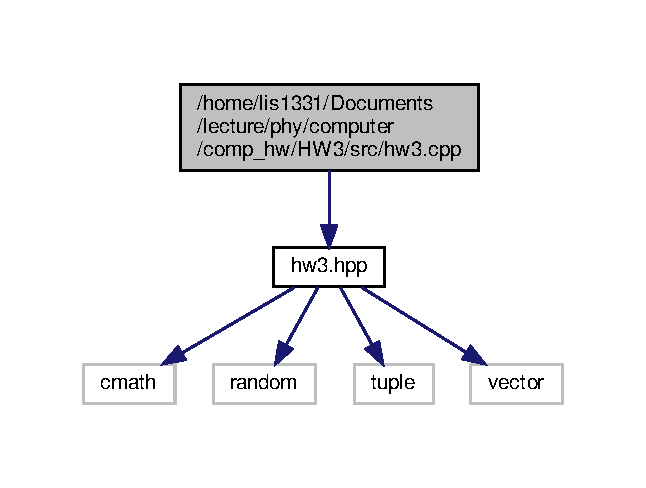
\includegraphics[width=310pt]{hw3_8cpp__incl}
\end{center}
\end{figure}
\subsection*{Functions}
\begin{DoxyCompactItemize}
\item 
\mbox{\Hypertarget{hw3_8cpp_a97f3fe0975c8f8646f2b42ee97163a81}\label{hw3_8cpp_a97f3fe0975c8f8646f2b42ee97163a81}} 
tuple$<$ double, vector$<$ double $>$, vector$<$ double $>$, vector$<$ double $>$ $>$ {\bfseries H\+W3} (double zeta\+\_\+min, double t0, int n, int num\+\_\+sine, int num\+\_\+iter, double step, mt19937 \&gen, uniform\+\_\+real\+\_\+distribution$<$ double $>$ \&dist)
\end{DoxyCompactItemize}


\subsection{Detailed Description}
code for homework3 of Computer1 class in Yonsei University Minimize the action by Markov Chain Monte Carlo Method to solve Kepler problem 

\begin{DoxyAuthor}{Author}
pistack (Junho Lee) 
\end{DoxyAuthor}
\begin{DoxyDate}{Date}
2021. 10. 10. 
\end{DoxyDate}

\hypertarget{hw3_8hpp}{}\section{/home/lis1331/\+Documents/lecture/phy/computer/comp\+\_\+hw/\+H\+W3/src/include/hw3.hpp File Reference}
\label{hw3_8hpp}\index{/home/lis1331/\+Documents/lecture/phy/computer/comp\+\_\+hw/\+H\+W3/src/include/hw3.\+hpp@{/home/lis1331/\+Documents/lecture/phy/computer/comp\+\_\+hw/\+H\+W3/src/include/hw3.\+hpp}}


headerfile for homework3 of Computer1 class in Yonsei University Minimize the action by Markov Chain Monte Carlo Method to solve Kepler problem  


{\ttfamily \#include $<$cmath$>$}\newline
{\ttfamily \#include $<$random$>$}\newline
{\ttfamily \#include $<$tuple$>$}\newline
{\ttfamily \#include $<$vector$>$}\newline
Include dependency graph for hw3.\+hpp\+:\nopagebreak
\begin{figure}[H]
\begin{center}
\leavevmode
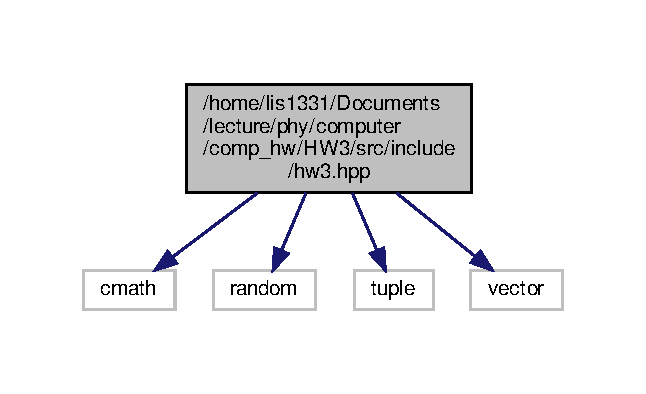
\includegraphics[width=310pt]{hw3_8hpp__incl}
\end{center}
\end{figure}
This graph shows which files directly or indirectly include this file\+:\nopagebreak
\begin{figure}[H]
\begin{center}
\leavevmode
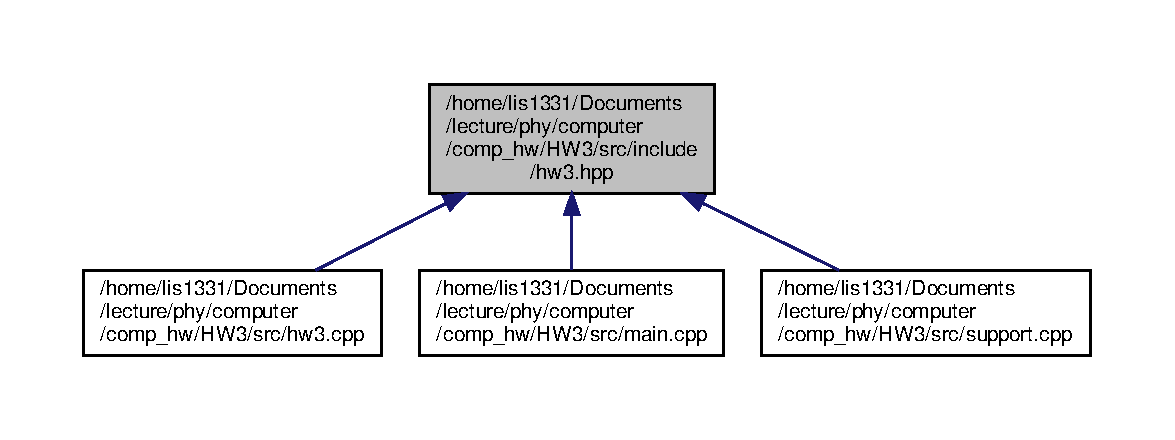
\includegraphics[width=350pt]{hw3_8hpp__dep__incl}
\end{center}
\end{figure}
\subsection*{Functions}
\begin{DoxyCompactItemize}
\item 
std\+::vector$<$ double $>$ \hyperlink{hw3_8hpp_a19af3e752398ebe136e7e9a02e758c41}{scale\+\_\+and\+\_\+add\+\_\+vector} (std\+::vector$<$ double $>$ \&v, double scale, double add)
\begin{DoxyCompactList}\small\item\em scale vector by scaler and add vector by adder \end{DoxyCompactList}\item 
std\+::tuple$<$ std\+::vector$<$ double $>$, std\+::vector$<$ double $>$ $>$ \hyperlink{hw3_8hpp_ac3be6003f22ac64d3e0028ba23a4fa7f}{sum\+\_\+of\+\_\+sine} (std\+::vector$<$ double $>$ \&t, std\+::vector$<$ double $>$ c, int num\+\_\+sine)
\begin{DoxyCompactList}\small\item\em evaluates sum of sine function with period 4$\ast$(t\+\_\+max-\/t\+\_\+min) weighted by coefficents and its derivative at given time t. \end{DoxyCompactList}\item 
std\+::vector$<$ double $>$ \hyperlink{hw3_8hpp_a062f905b73ecff0f68817abde17156a2}{move\+\_\+step} (std\+::vector$<$ double $>$ \&init\+\_\+guess, double step, std\+::mt19937 \&gen, std\+::uniform\+\_\+real\+\_\+distribution$<$ double $>$ \&dist)
\begin{DoxyCompactList}\small\item\em randomly move initial guess by step \end{DoxyCompactList}\item 
double \hyperlink{hw3_8hpp_aadb1c96f9250fd3017d55a03d6e3c80f}{eval\+\_\+action} (std\+::vector$<$ double $>$ \&t, std\+::vector$<$ double $>$ zeta, std\+::vector$<$ double $>$ deriv\+\_\+zeta, std\+::vector$<$ double $>$ theta, std\+::vector$<$ double $>$ deriv\+\_\+theta)
\begin{DoxyCompactList}\small\item\em evaluates the action of given path \end{DoxyCompactList}\item 
std\+::tuple$<$ double, std\+::vector$<$ double $>$, std\+::vector$<$ double $>$, std\+::vector$<$ double $>$ $>$ \hyperlink{hw3_8hpp_ac216313e859231319b1d893df8bcba01}{H\+W3} (double zeta\+\_\+min, double t0, int n, int num\+\_\+sine, int num\+\_\+iter, double step, std\+::mt19937 \&gen, std\+::uniform\+\_\+real\+\_\+distribution$<$ double $>$ \&dist)
\begin{DoxyCompactList}\small\item\em H\+W3\+: Solve Kepler problem via Markov Chain Monte Carlo Method see H\+W3.\+pdf for further detail. \end{DoxyCompactList}\end{DoxyCompactItemize}
\subsection*{Variables}
\begin{DoxyCompactItemize}
\item 
\mbox{\Hypertarget{hw3_8hpp_a43016d873124d39034edb8cd164794db}\label{hw3_8hpp_a43016d873124d39034edb8cd164794db}} 
const double {\bfseries pi} = 3.\+141592653589793
\end{DoxyCompactItemize}


\subsection{Detailed Description}
headerfile for homework3 of Computer1 class in Yonsei University Minimize the action by Markov Chain Monte Carlo Method to solve Kepler problem 

\begin{DoxyAuthor}{Author}
pistack (Junho Lee) 
\end{DoxyAuthor}
\begin{DoxyDate}{Date}
2021. 10. 10. 
\end{DoxyDate}


\subsection{Function Documentation}
\mbox{\Hypertarget{hw3_8hpp_aadb1c96f9250fd3017d55a03d6e3c80f}\label{hw3_8hpp_aadb1c96f9250fd3017d55a03d6e3c80f}} 
\index{hw3.\+hpp@{hw3.\+hpp}!eval\+\_\+action@{eval\+\_\+action}}
\index{eval\+\_\+action@{eval\+\_\+action}!hw3.\+hpp@{hw3.\+hpp}}
\subsubsection{\texorpdfstring{eval\+\_\+action()}{eval\_action()}}
{\footnotesize\ttfamily double eval\+\_\+action (\begin{DoxyParamCaption}\item[{std\+::vector$<$ double $>$ \&}]{t,  }\item[{std\+::vector$<$ double $>$}]{zeta,  }\item[{std\+::vector$<$ double $>$}]{deriv\+\_\+zeta,  }\item[{std\+::vector$<$ double $>$}]{theta,  }\item[{std\+::vector$<$ double $>$}]{deriv\+\_\+theta }\end{DoxyParamCaption})}



evaluates the action of given path 


\begin{DoxyParams}{Parameters}
{\em t} & time \\
\hline
{\em zeta} & zeta part of path \\
\hline
{\em deriv\+\_\+zeta} & derivative of path, zeta part \\
\hline
{\em theta} & theta part of path \\
\hline
{\em deriv\+\_\+theta} & derivative of path, theta part \\
\hline
\end{DoxyParams}
\begin{DoxyReturn}{Returns}
the action of given path 
\end{DoxyReturn}
\mbox{\Hypertarget{hw3_8hpp_ac216313e859231319b1d893df8bcba01}\label{hw3_8hpp_ac216313e859231319b1d893df8bcba01}} 
\index{hw3.\+hpp@{hw3.\+hpp}!H\+W3@{H\+W3}}
\index{H\+W3@{H\+W3}!hw3.\+hpp@{hw3.\+hpp}}
\subsubsection{\texorpdfstring{H\+W3()}{HW3()}}
{\footnotesize\ttfamily std\+::tuple$<$double,std\+::vector$<$double$>$,std\+::vector$<$double$>$,std\+::vector$<$double$>$ $>$ H\+W3 (\begin{DoxyParamCaption}\item[{double}]{zeta\+\_\+min,  }\item[{double}]{t0,  }\item[{int}]{n,  }\item[{int}]{num\+\_\+sine,  }\item[{int}]{num\+\_\+iter,  }\item[{double}]{step,  }\item[{std\+::mt19937 \&}]{gen,  }\item[{std\+::uniform\+\_\+real\+\_\+distribution$<$ double $>$ \&}]{dist }\end{DoxyParamCaption})}



H\+W3\+: Solve Kepler problem via Markov Chain Monte Carlo Method see H\+W3.\+pdf for further detail. 


\begin{DoxyParams}{Parameters}
{\em zeta\+\_\+min} & minimum value of zeta, for constraint motion 0.\+5 $<$ zeta\+\_\+min $<$ 1 \\
\hline
{\em t0} & initial time \\
\hline
{\em n} & number of points to evaluate \\
\hline
{\em num\+\_\+sine} & number of sine functions to guess \\
\hline
{\em num\+\_\+iter} & number of iteration \\
\hline
{\em step} & step size \\
\hline
{\em gen} & random number generator (assume mt19937) \\
\hline
{\em dist} & distribution \\
\hline
\end{DoxyParams}
\begin{DoxyReturn}{Returns}
tuple of minimum action, time and path(zeta, theta) 
\end{DoxyReturn}
\mbox{\Hypertarget{hw3_8hpp_a062f905b73ecff0f68817abde17156a2}\label{hw3_8hpp_a062f905b73ecff0f68817abde17156a2}} 
\index{hw3.\+hpp@{hw3.\+hpp}!move\+\_\+step@{move\+\_\+step}}
\index{move\+\_\+step@{move\+\_\+step}!hw3.\+hpp@{hw3.\+hpp}}
\subsubsection{\texorpdfstring{move\+\_\+step()}{move\_step()}}
{\footnotesize\ttfamily std\+::vector$<$double$>$ move\+\_\+step (\begin{DoxyParamCaption}\item[{std\+::vector$<$ double $>$ \&}]{init\+\_\+guess,  }\item[{double}]{step,  }\item[{std\+::mt19937 \&}]{gen,  }\item[{std\+::uniform\+\_\+real\+\_\+distribution$<$ double $>$ \&}]{dist }\end{DoxyParamCaption})}



randomly move initial guess by step 


\begin{DoxyParams}{Parameters}
{\em init\+\_\+guess} & initial guess \\
\hline
{\em step} & step size\textbackslash{} \\
\hline
{\em gen} & random number generator (assume mt19937) \\
\hline
{\em dist} & distribution \\
\hline
\end{DoxyParams}
\begin{DoxyReturn}{Returns}
moved initial guess by step 
\end{DoxyReturn}
\mbox{\Hypertarget{hw3_8hpp_a19af3e752398ebe136e7e9a02e758c41}\label{hw3_8hpp_a19af3e752398ebe136e7e9a02e758c41}} 
\index{hw3.\+hpp@{hw3.\+hpp}!scale\+\_\+and\+\_\+add\+\_\+vector@{scale\+\_\+and\+\_\+add\+\_\+vector}}
\index{scale\+\_\+and\+\_\+add\+\_\+vector@{scale\+\_\+and\+\_\+add\+\_\+vector}!hw3.\+hpp@{hw3.\+hpp}}
\subsubsection{\texorpdfstring{scale\+\_\+and\+\_\+add\+\_\+vector()}{scale\_and\_add\_vector()}}
{\footnotesize\ttfamily std\+::vector$<$double$>$ scale\+\_\+and\+\_\+add\+\_\+vector (\begin{DoxyParamCaption}\item[{std\+::vector$<$ double $>$ \&}]{v,  }\item[{double}]{scale,  }\item[{double}]{add }\end{DoxyParamCaption})}



scale vector by scaler and add vector by adder 


\begin{DoxyParams}{Parameters}
{\em v} & vector to scale and add \\
\hline
{\em scale} & scaler \\
\hline
{\em add} & adder \\
\hline
\end{DoxyParams}
\begin{DoxyReturn}{Returns}
scale and added vector (scale$\ast$v+add) 
\end{DoxyReturn}
\mbox{\Hypertarget{hw3_8hpp_ac3be6003f22ac64d3e0028ba23a4fa7f}\label{hw3_8hpp_ac3be6003f22ac64d3e0028ba23a4fa7f}} 
\index{hw3.\+hpp@{hw3.\+hpp}!sum\+\_\+of\+\_\+sine@{sum\+\_\+of\+\_\+sine}}
\index{sum\+\_\+of\+\_\+sine@{sum\+\_\+of\+\_\+sine}!hw3.\+hpp@{hw3.\+hpp}}
\subsubsection{\texorpdfstring{sum\+\_\+of\+\_\+sine()}{sum\_of\_sine()}}
{\footnotesize\ttfamily std\+::tuple$<$std\+::vector$<$double$>$, std\+::vector$<$double$>$ $>$ sum\+\_\+of\+\_\+sine (\begin{DoxyParamCaption}\item[{std\+::vector$<$ double $>$ \&}]{t,  }\item[{std\+::vector$<$ double $>$}]{c,  }\item[{int}]{num\+\_\+sine }\end{DoxyParamCaption})}



evaluates sum of sine function with period 4$\ast$(t\+\_\+max-\/t\+\_\+min) weighted by coefficents and its derivative at given time t. 


\begin{DoxyParams}{Parameters}
{\em t} & time \\
\hline
{\em c} & coefficiets \\
\hline
{\em num\+\_\+sine} & number of sine function to add \\
\hline
\end{DoxyParams}
\begin{DoxyReturn}{Returns}
tuple of value and derivatives of the sum of sine function 
\end{DoxyReturn}

\hypertarget{main_8cpp}{}\section{/home/lis1331/\+Documents/lecture/phy/computer/comp\+\_\+hw/\+H\+W3/src/main.cpp File Reference}
\label{main_8cpp}\index{/home/lis1331/\+Documents/lecture/phy/computer/comp\+\_\+hw/\+H\+W3/src/main.\+cpp@{/home/lis1331/\+Documents/lecture/phy/computer/comp\+\_\+hw/\+H\+W3/src/main.\+cpp}}


main program for homework3 of Computer1 class in Yonsei University Interactively reads inital condition, number of sine function used for guess, number of gird points to evaluate, number of interation, step size and output file name then computes and saves solution.  


{\ttfamily \#include $<$string$>$}\newline
{\ttfamily \#include $<$iostream$>$}\newline
{\ttfamily \#include $<$fstream$>$}\newline
{\ttfamily \#include \char`\"{}hw3.\+hpp\char`\"{}}\newline
Include dependency graph for main.\+cpp\+:\nopagebreak
\begin{figure}[H]
\begin{center}
\leavevmode
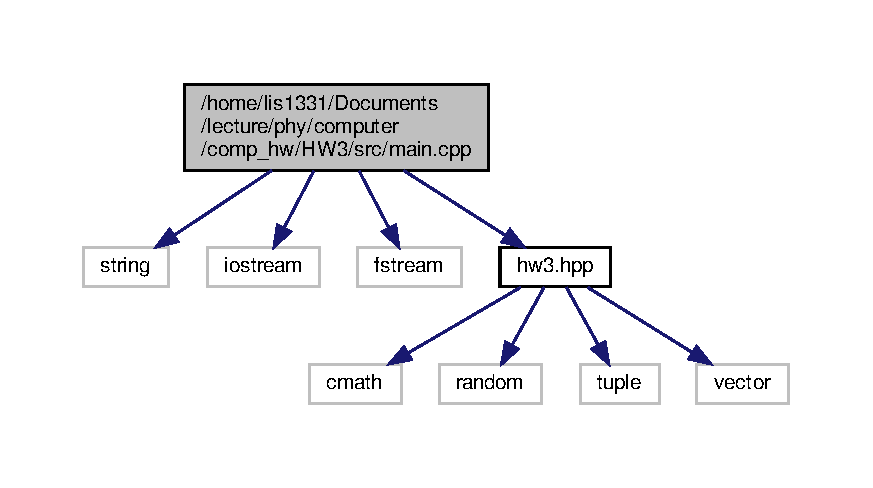
\includegraphics[width=350pt]{main_8cpp__incl}
\end{center}
\end{figure}
\subsection*{Functions}
\begin{DoxyCompactItemize}
\item 
\mbox{\Hypertarget{main_8cpp_a840291bc02cba5474a4cb46a9b9566fe}\label{main_8cpp_a840291bc02cba5474a4cb46a9b9566fe}} 
int {\bfseries main} (void)
\end{DoxyCompactItemize}


\subsection{Detailed Description}
main program for homework3 of Computer1 class in Yonsei University Interactively reads inital condition, number of sine function used for guess, number of gird points to evaluate, number of interation, step size and output file name then computes and saves solution. 

\begin{DoxyAuthor}{Author}
pistack (Junho Lee) 
\end{DoxyAuthor}
\begin{DoxyDate}{Date}
2021. 10. 10. 
\end{DoxyDate}

\hypertarget{support_8cpp}{}\section{/home/lis1331/\+Documents/lecture/phy/computer/comp\+\_\+hw/\+H\+W3/src/support.cpp File Reference}
\label{support_8cpp}\index{/home/lis1331/\+Documents/lecture/phy/computer/comp\+\_\+hw/\+H\+W3/src/support.\+cpp@{/home/lis1331/\+Documents/lecture/phy/computer/comp\+\_\+hw/\+H\+W3/src/support.\+cpp}}


support functions for homework3 of Computer1 class in Yonsei University scale and add vector, evaluate sum and derivative of sine function, randomly move initial guess by step and evaluate the action of given path.  


{\ttfamily \#include \char`\"{}hw3.\+hpp\char`\"{}}\newline
Include dependency graph for support.\+cpp\+:\nopagebreak
\begin{figure}[H]
\begin{center}
\leavevmode
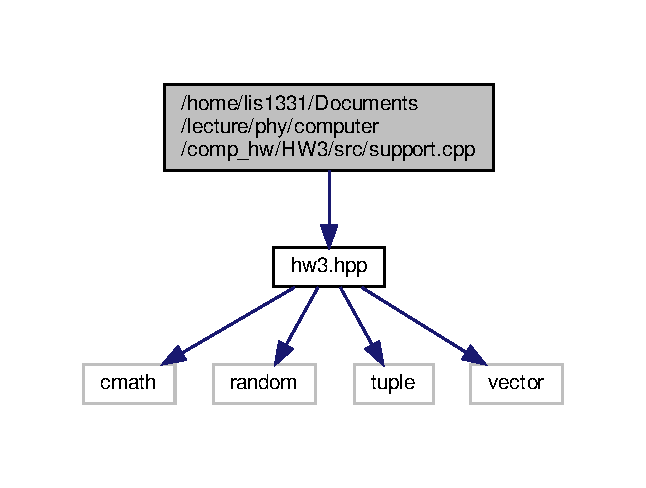
\includegraphics[width=310pt]{support_8cpp__incl}
\end{center}
\end{figure}
\subsection*{Functions}
\begin{DoxyCompactItemize}
\item 
\mbox{\Hypertarget{support_8cpp_a33f3d8de61c49e3251c5d58b3b3f97a9}\label{support_8cpp_a33f3d8de61c49e3251c5d58b3b3f97a9}} 
vector$<$ double $>$ {\bfseries scale\+\_\+and\+\_\+add\+\_\+vector} (vector$<$ double $>$ \&v, double scale, double add)
\item 
\mbox{\Hypertarget{support_8cpp_a4e7773ac6ed19ce46e8bd242eecf450f}\label{support_8cpp_a4e7773ac6ed19ce46e8bd242eecf450f}} 
tuple$<$ vector$<$ double $>$, vector$<$ double $>$ $>$ {\bfseries sum\+\_\+of\+\_\+sine} (vector$<$ double $>$ \&t, vector$<$ double $>$ c, int num\+\_\+sine)
\item 
\mbox{\Hypertarget{support_8cpp_ab27932438b60b5d027874f2f964d8ad0}\label{support_8cpp_ab27932438b60b5d027874f2f964d8ad0}} 
vector$<$ double $>$ {\bfseries move\+\_\+step} (vector$<$ double $>$ \&init\+\_\+guess, double step, mt19937 \&gen, uniform\+\_\+real\+\_\+distribution$<$ double $>$ \&dist)
\item 
\mbox{\Hypertarget{support_8cpp_a7a7182652d0cca7186208c1f96fe2923}\label{support_8cpp_a7a7182652d0cca7186208c1f96fe2923}} 
double {\bfseries eval\+\_\+action} (vector$<$ double $>$ \&t, vector$<$ double $>$ zeta, vector$<$ double $>$ deriv\+\_\+zeta, vector$<$ double $>$ theta, vector$<$ double $>$ deriv\+\_\+theta)
\end{DoxyCompactItemize}


\subsection{Detailed Description}
support functions for homework3 of Computer1 class in Yonsei University scale and add vector, evaluate sum and derivative of sine function, randomly move initial guess by step and evaluate the action of given path. 

\begin{DoxyAuthor}{Author}
pistack (Junho Lee) 
\end{DoxyAuthor}
\begin{DoxyDate}{Date}
2021. 10. 10. 
\end{DoxyDate}

%--- End generated contents ---

% Index
\backmatter
\newpage
\phantomsection
\clearemptydoublepage
\addcontentsline{toc}{chapter}{Index}
\printindex

\end{document}
